\section{Experimental Results}
\label{sec:experimental_results}
In the following section summarizes the results from experiments with the soft manipulator. We discuss the grasping of delicate objects and cylindrical objects as well as the repeatability and success rate of the autonomous system.
 
\subsection{Grasping Delicate Objects}
\rkk{It was shown in \cite{marchese2015recipe} that pleated grippers of similar dimensions like the one used in this work can exert a continuous spectrum of blocking force in the range of 0-2\unit{N} at a pressure range of 0-60\unit{kPa}. Grasping delicate objects should therefore be possible with the soft manipulator.}
The manipulator in fact picks up delicate objects \rkk{such as eggs, shuttlecocks or bakery items} without \rkk{squishing} or breaking those. 
Figure~\ref{fig:egg_approach_sequence} shows how the manipulator approaches and grasps an egg.
Delicate objects can be manipulated without requiring a shape or a force sensor within its structure, since the compliant gripper body conforms to the object.
Rigid-bodied grippers usually rely on force sensing or another type of sensory feedback to avoid damage caused to the object.

\begin{figure}[htb]
\centering
   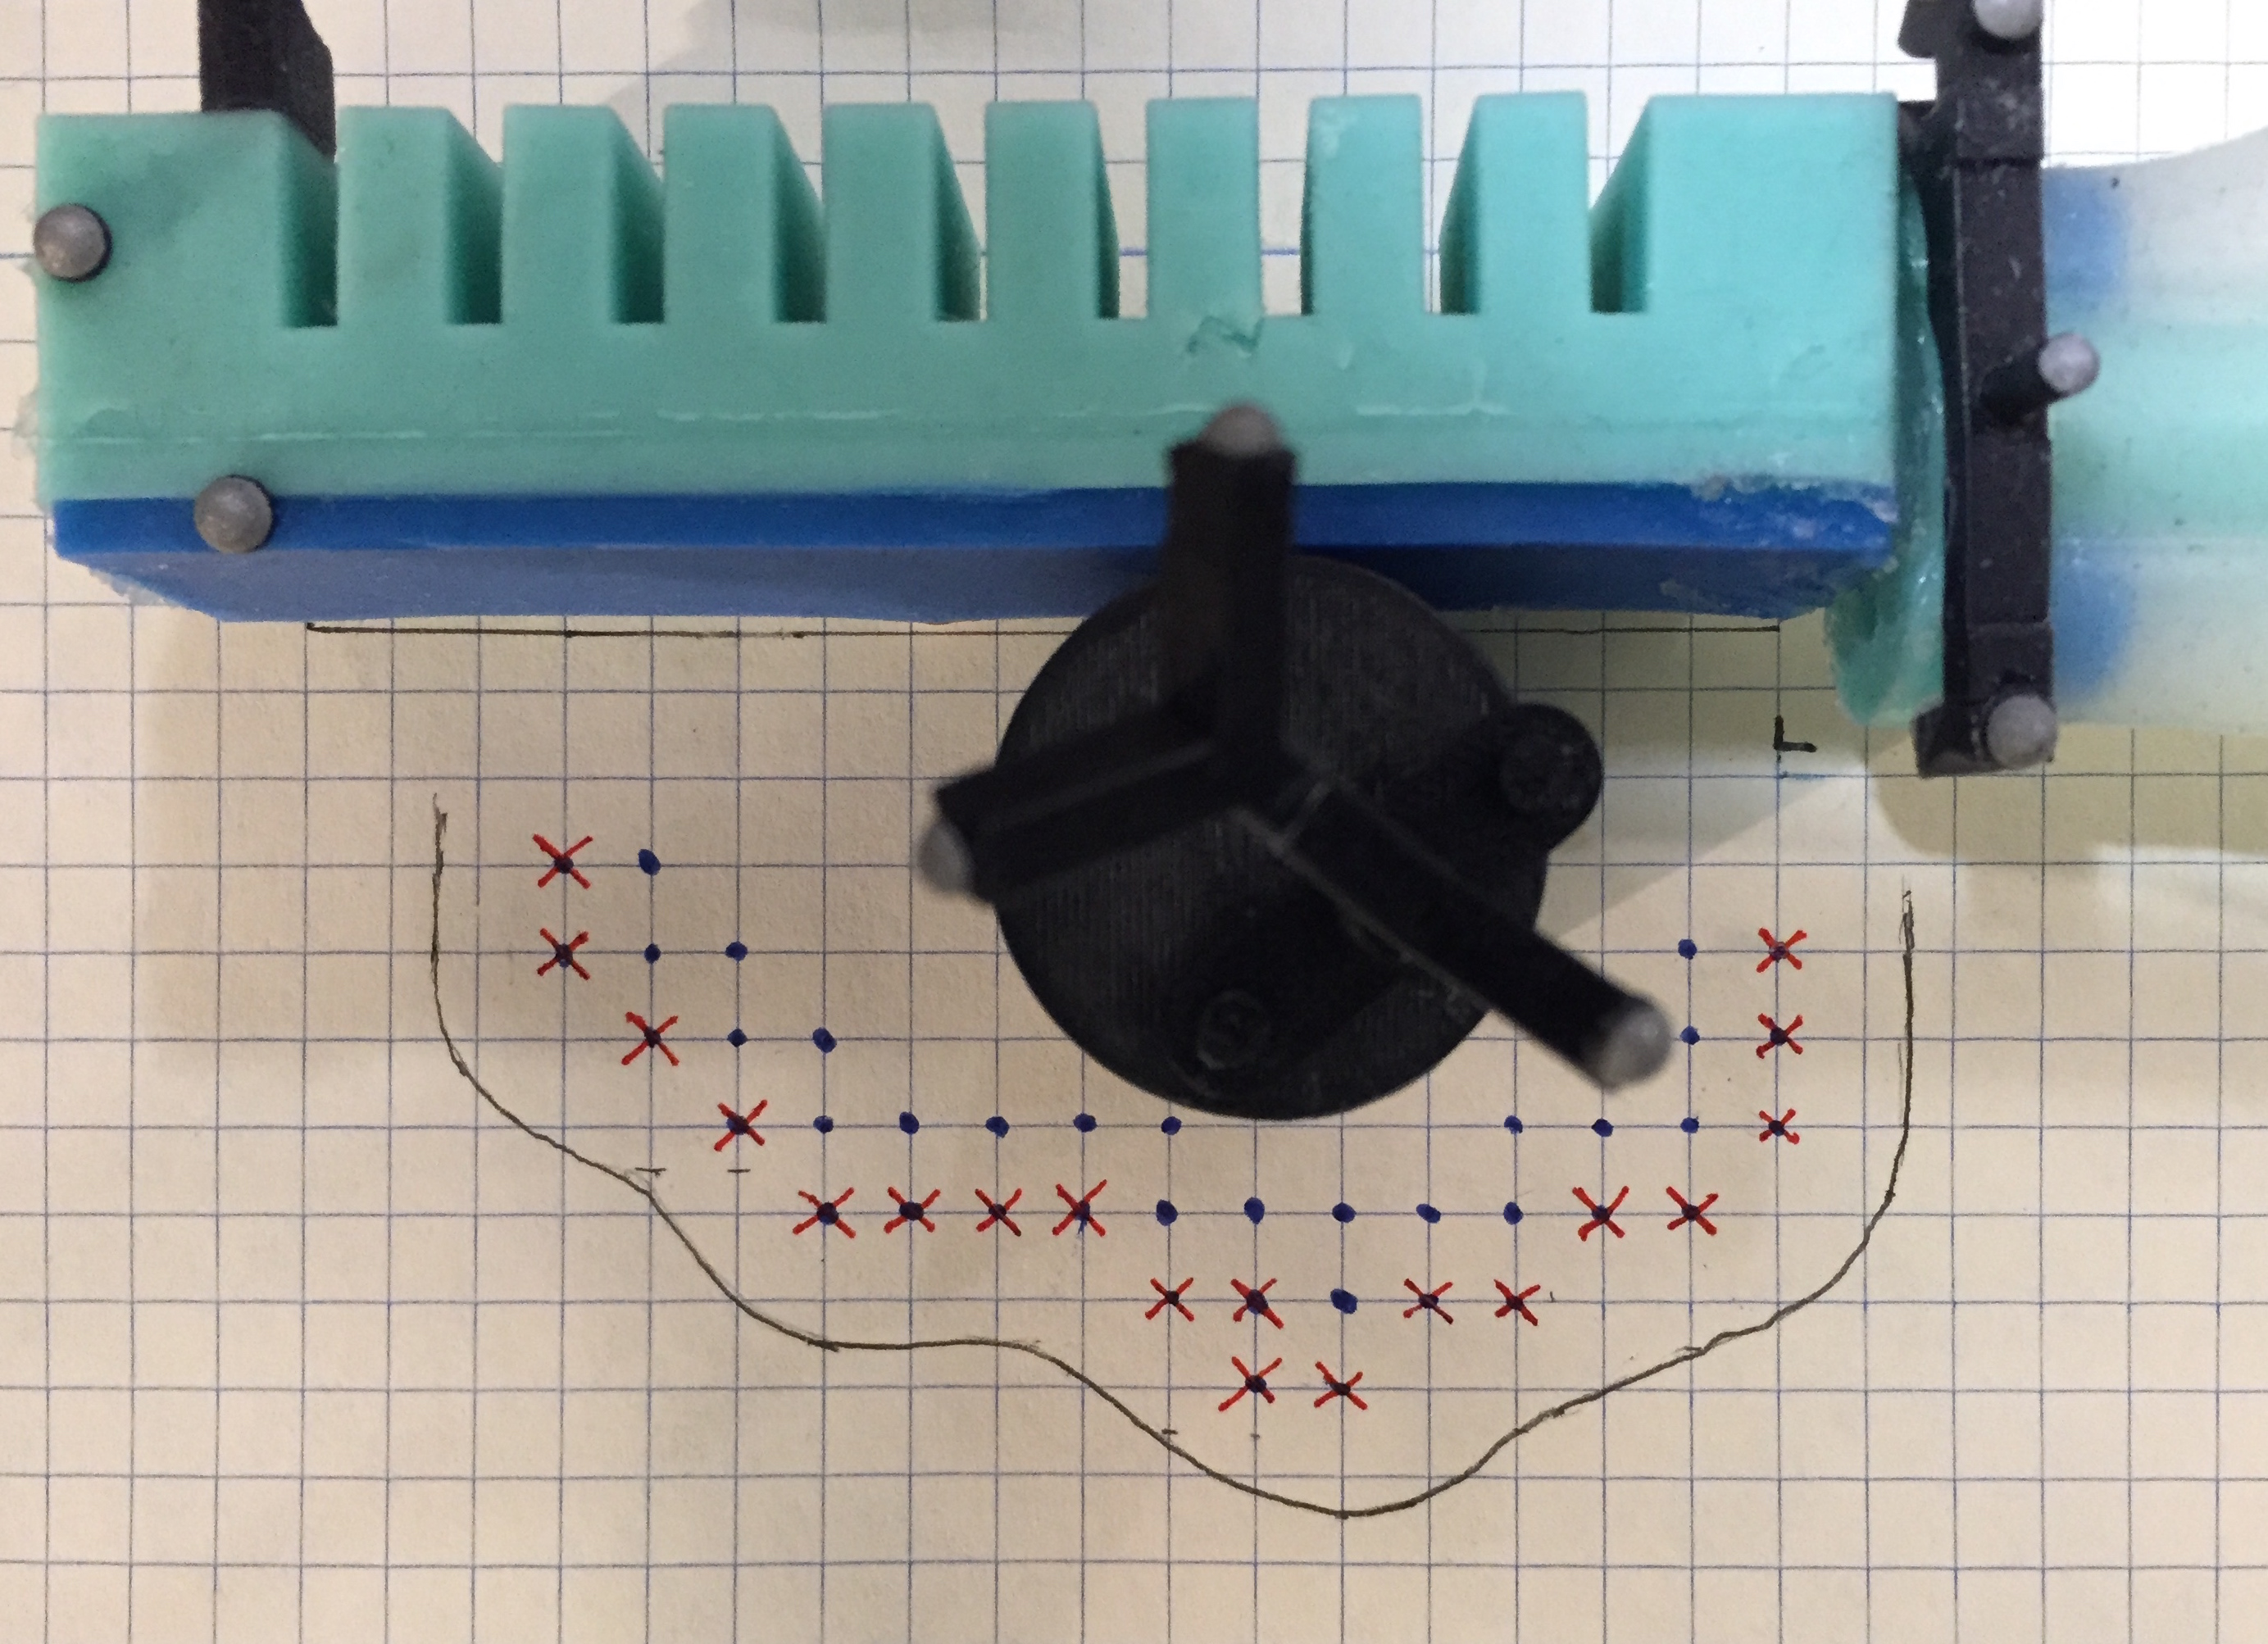
\includegraphics[width=0.8\columnwidth]{Figures/experimental_results/uncertainty}
   \caption{Experimental characterization of the gripper's capture region: the allowable positioning uncertainty is determined through repeated placements of the center of a cylindrical object at different points on a grid relative to the gripper. Blue dots indicate all object center positions for which a grasp could be performed successfully, red crosses show the positions where a grasp failed. The grey line outlines an area for the object to be positioned within so the gripper can grasp it. The evaluation of the capture region was performed similarly to a method described in \cite{dogar2010push}.}
   \label{fig:grasp_uncertainty}
\end{figure} 

\subsection{Repeated Grasp Experiments}
We performed 25 experimental grasp-and-place trials at various positions to demonstrate the capabilities and repeatability of our system.
The results of all the trials are shown in Figure~\ref{fig:allTestsOverlaid}.
One representative approach, grasp, and retract move is shown in Figure~\ref{fig:oneTrialVsTime}.
In 23 of 25 experimental trials, the manipulator successfully achieved the task of grasping an object and bringing it to a bin location shown in red.
The object was placed five times on each of the five points marked on the board.
The markers only serve as a reference point for the user to place the object roughly at the same point at every repetition.
The user's placing accuracy is not important to the algorithm, the tracking system newly registers every single time the position of the placed object.
The five points were chosen to approximately represent the major portion of the manipulator's reachable workspace.
As long as the root of the gripper stops so that the object is located within the capture region, the gripper will pick it up through its sweeping closing motion. The capture region is shown in grey in Figure~\ref{fig:grasp_uncertainty}. 
The evaluation of the capture region is performed similarly to a method described in Dogar and Srinivasa\cite{dogar2010push} work on determining capture regions for a push-grasp of a classical robotic gripper.
\rkk{Grid paper and fine markings on all four sides of the round object ensure that the placement by the user is accurate within $\pm$1\unit{mm} in relation to the discrete placement locations on the grid. This test serves as a qualitative measure to show a relation between object size to gripper size to area of successful grasp.}
Despite positioning inaccuracies of the soft manipulator, the gripper can nevertheless successfully perform a grasp of an object. 

When the arm reaches \rkk{its straight pose within a relatively large delta}, it drops the object.
\rkk{For these experiments, we focus on showing the capability of picking up objects at various places and moving them around, there is no emphasis set on having to drop off the object at a specific pose. To indicate that the arm can move the object after grasping, the arm was controlled to go back to the fully straight pose. When it got fairly close to that final straight pose within a large allowable delta, the gripper was set to release and drop the object. It was not ensured by the planner that the arm had to first settle to zero velocity at the final straight pose. As a consequence of this, the experimental data indicates as a red bin a relatively wide drop off area.}

\begin{figure*}[htbp]
\begin{centering}
  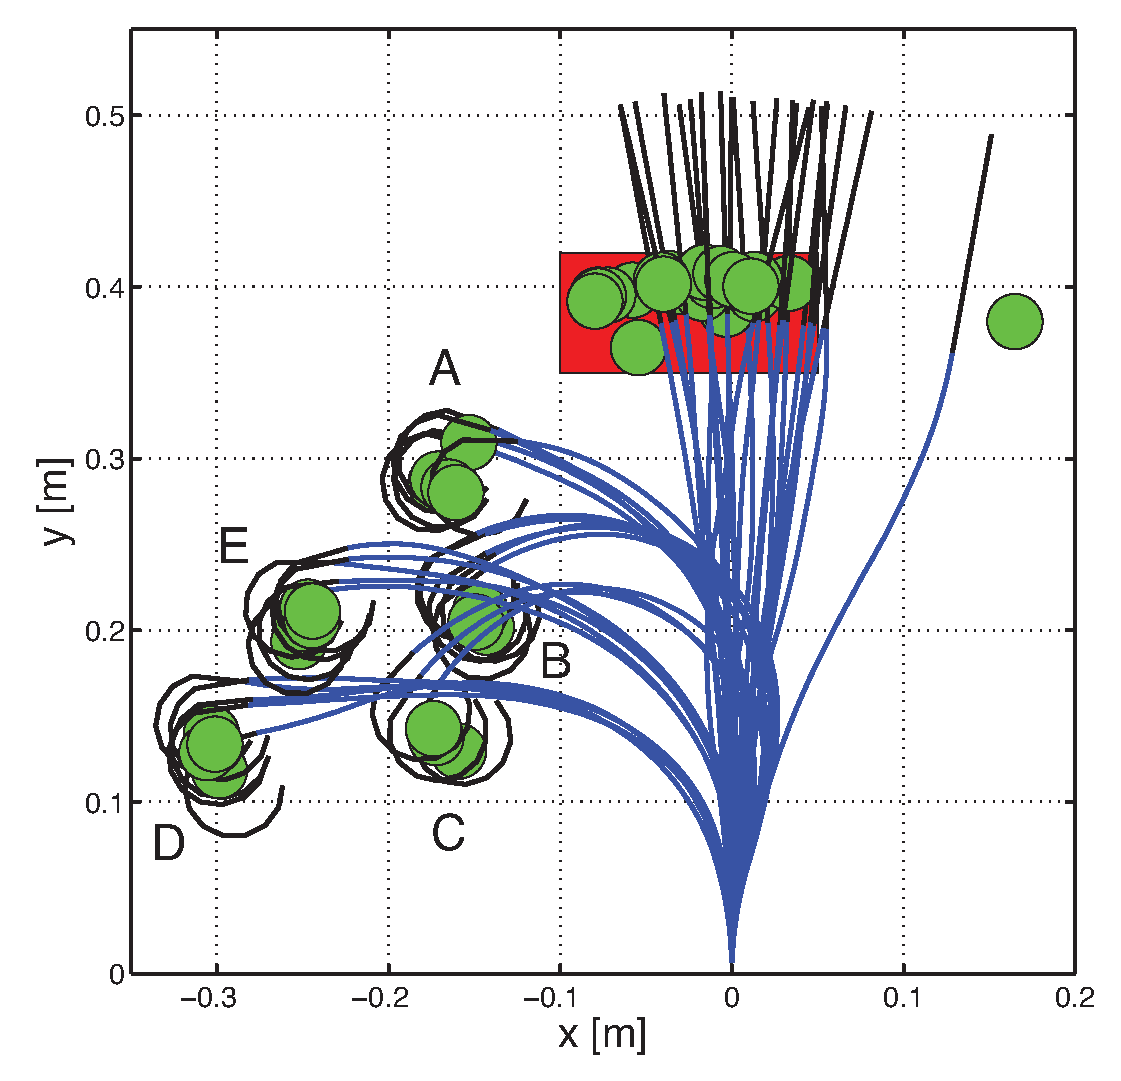
\includegraphics[width=0.5\textwidth]{Figures/experimental_results/allTestsOverlaid.eps}
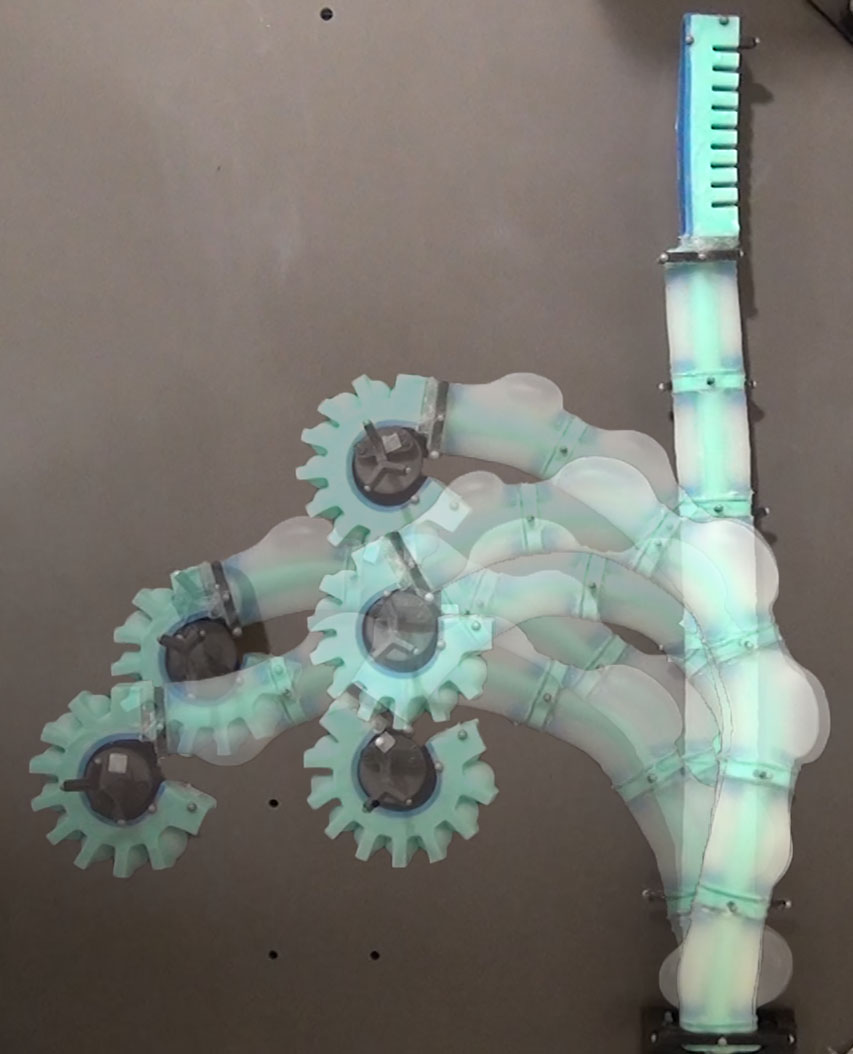
\includegraphics[width=0.385\textwidth]{figures/experimental_results/five_grasps.jpg}
\caption[Left: All 25 experimental grasping trials.]{Complete set of experimental grasp-and-place trials. In these experiments, the arm moves from an initial straightened configuration to grasp a round object placed in one of five locations (A-E). The arm then returns the object to a bin location shown in red. For each trial, a seven degrees of freedom manipulator representation is generated at both the \emph{grasped} and \emph{released} state using experimental data and is shown in blue. The corresponding 1 degree-of-freedom end-effector representation is shown in black. The round object's measured position at each state is shown in green. Right: Overlaid photographs of the manipulator grasping an object placed at each of the five locations. }\label{fig:allTestsOverlaid}
\end{centering}
\end{figure*}

The unsuccessful trials happened due to stick-slip friction between the roller bearings and the table surface.
Our kinematic modeling does not account for this non-linear behavior, which acts as a disturbance and can lead to failure to arrive at the next waypoint.
To be more specific, in one of the trials, the robot slowed down too much before it almost reached its next waypoint and because of friction the arm halted to a full stop. 
The proportional gain of the curvature controller was not able to compensate for that small positional delta and since the relatively low saturation level of the integrator portion of the controller was saturated, the arm did not move to the next waypoint pose. 
It is to note, that the saturation level for the integrator is defined by a safety limit on the maximal inflation of the robotic arm.
In the other unsuccesful trial, the stick-slip friction also caused the arm to halt before a waypoint. The controller built up enough forcing due to inflation, so that the arm slipped over the close waypoint without having all of its single arm segment curvature within an acceptable epsilon.
The controller then tried to swing back to fulfill the missed waypoint, missed it again and that finally caused the whole arm to oscillate back-and-forth and eventually push the object off the table.
In one of the other trials, the grasp and return was successfully performed, but a small overshoot over the final bin location at the end of the return caused the arm to drop off the table, which could have been avoided if the table would have not been too small towards the right.
This outlier is shown in Figure~\ref{fig:allTestsOverlaid}.
Overall, the experiments show that the system was repeatably able to autonomously locate a randomly placed object within its workspace, plan the arm motions, and perform the task of grasping and placing the object.

\subsection{Experimental Insights and Limitations}
The system can drag payloads of less than 40\unit{g}, higher payloads cause the cylindrical arm segments to stall and possibly lift off the table without moving the payload.
There is a trade-off between the reachable workspace and the maximum payload.
As the length of the arm increases, more workspace can be reached while less payload can be manipulated. 
Most of the payload capability is already used up by the attached gripper itself.
A smaller gripper would allow for larger payloads to get picked up, but consequently only smaller objects can be grasped.
The workspace of the manipulator is limited to the top and left by the maximal extension length of the arm, and to the bottom by the maximum bending curvature, which the arm can achieve without over-actuating a single segment.
\rkk{The gripper presented can not only pick up a round object, but also more arbitrarily shaped objects of similar size, for example a star-shaped object, a tape holder, a shuttlecock or an egg.}
Objects were only grasped within the left quadrant of the arm, because of the gripper orientation and an upright initial starting pose.
\rkk{A smoothing of the complete trajectory with several intermediate waypoints was found to be necessary. The amount of intermediate waypoints is determined by the variable $\delta d$, which we found empirically to be 5\unit{cm}, around half the length of the gripper. A new waypoint is sent to the controller immediately after arriving within a small delta of the previous waypoint, the controllers for each arm segment then compensate for the new delta in curvature as quickly as possible to get to the new pose $\kappa_i^*$.}
\rkk{The instabilities observed in the unsuccessful trials could be solved by loosening the constraints on the planner. The planner could allow the arm controller to have the arm pass over each intermediate waypoint without having to get to a full stop within an arbitrarily chosen delta of curvature values. The planner could take as a measure of progress a decreasing cartesian distance of the gripper to its final target pose.}
\rkk{It is worth mentioning that the exteroceptive tracking system has the disadvantage that an occlusion of one or more markers can cause the tracking system to temporarily loose track of a measured arm segment. In that case, the control loop can not function properly until the occlusion disappears. Proprioceptive sensors within the segments can solve this issue.}

\begin{figure*}[htbp]
\begin{centering}
  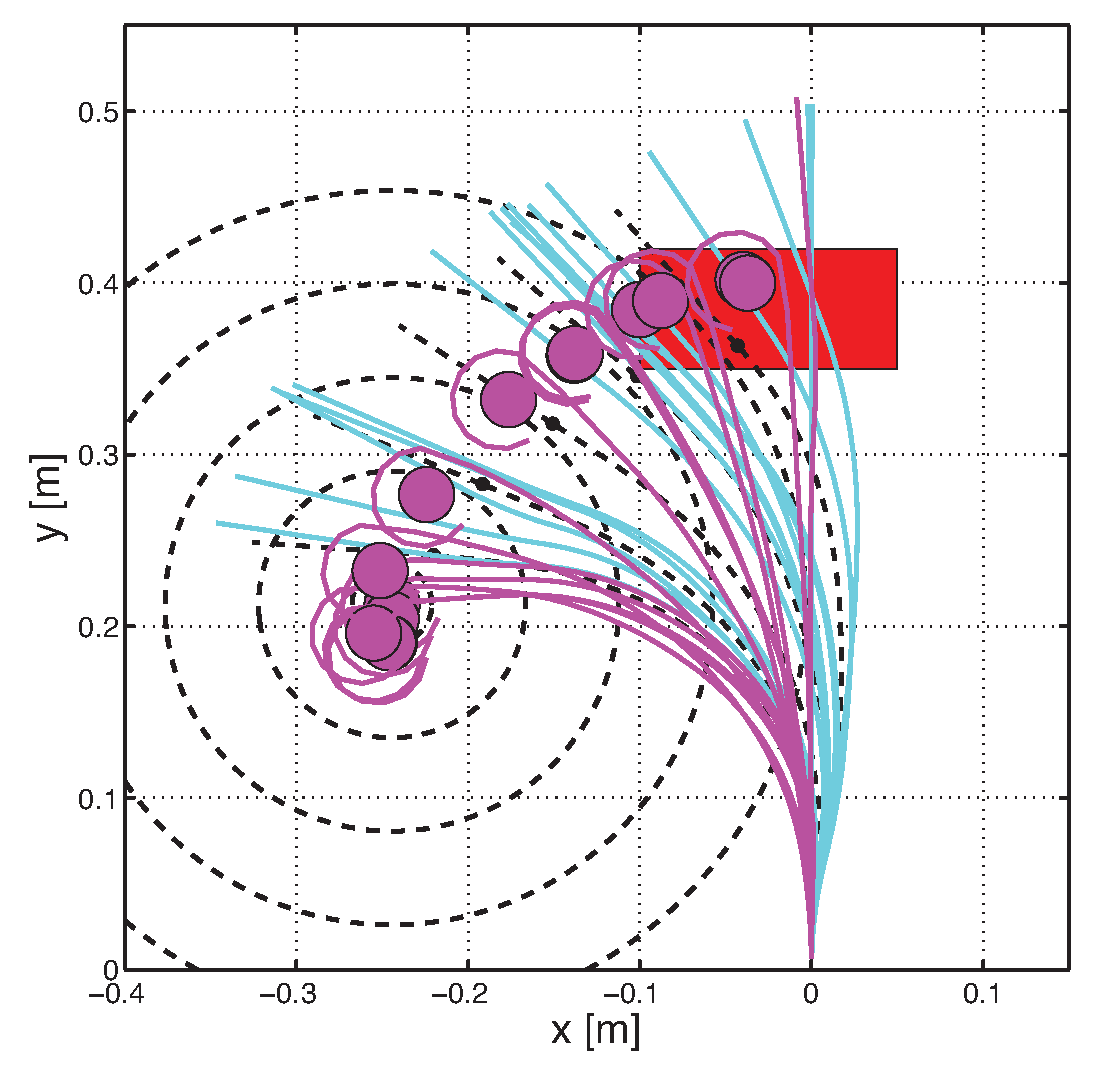
\includegraphics[width=0.375\textwidth]{Figures/experimental_results/oneTrialVsTime.eps}
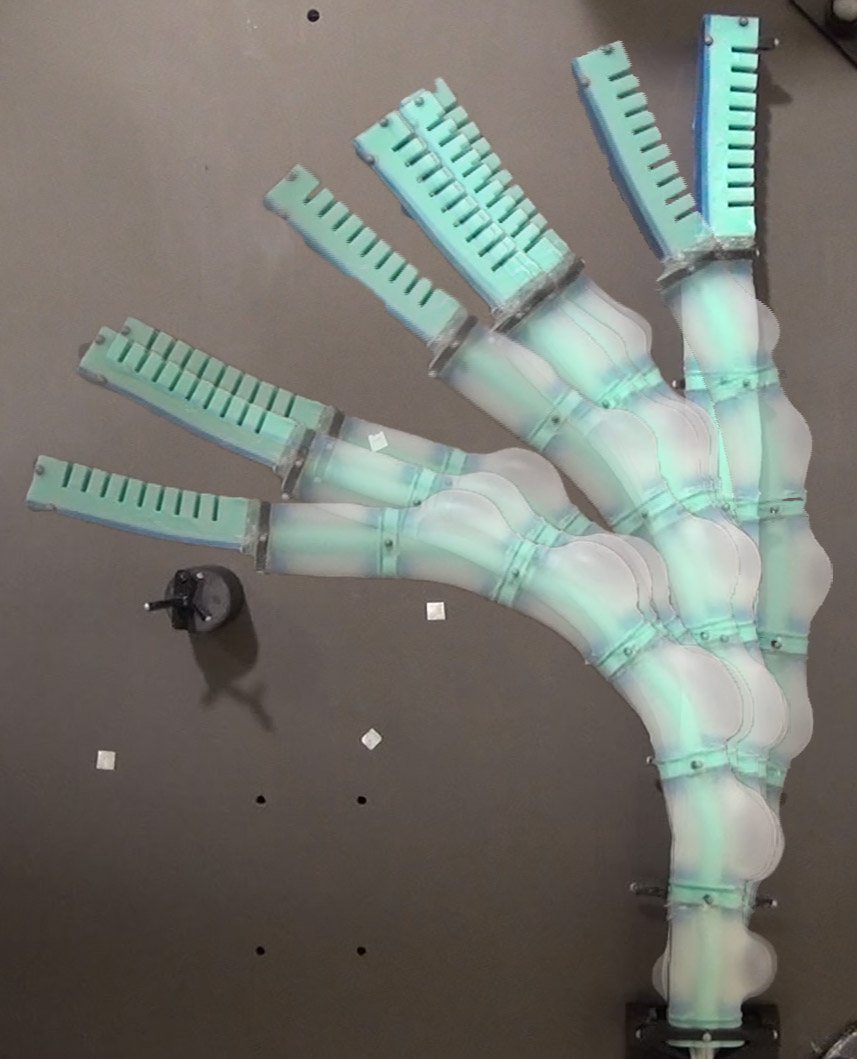
\includegraphics[width=0.30\textwidth]{figures/experimental_results/exp5a-4_sweep_to_object.jpg}
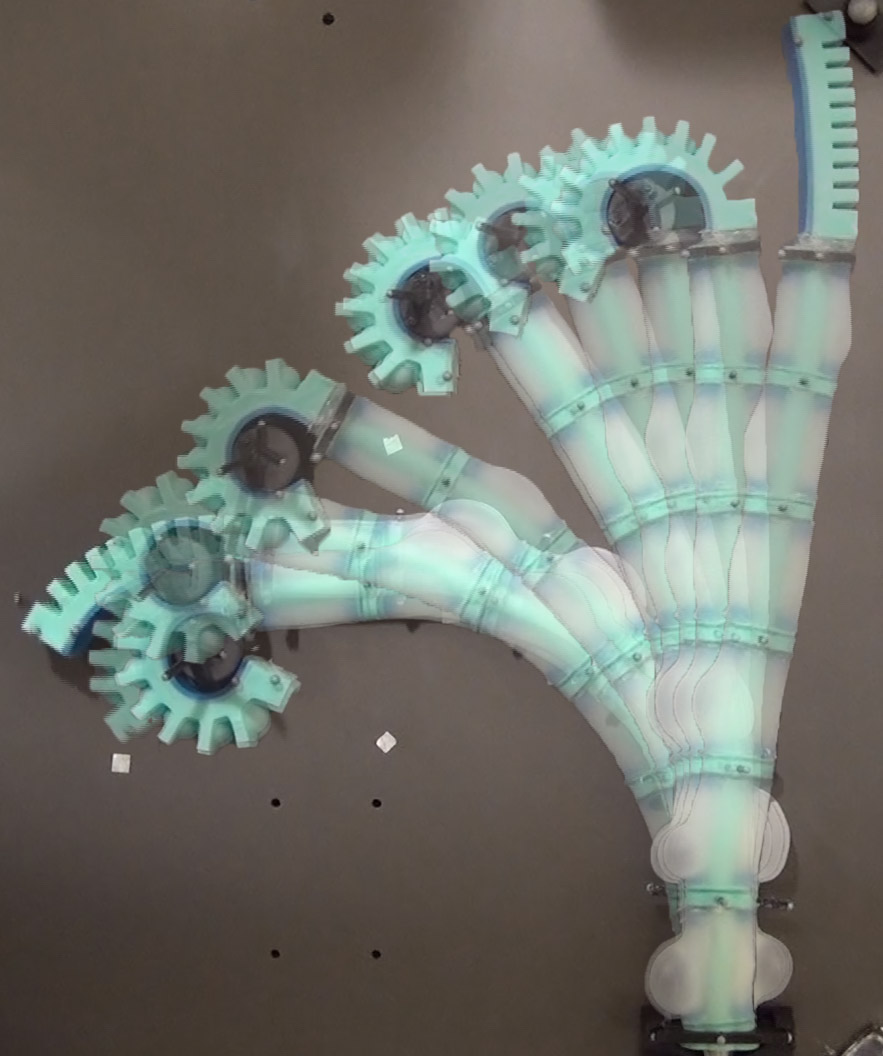
\includegraphics[width=0.31\textwidth]{figures/experimental_results/exp5a-4_sweep_to_bin.jpg}
  \caption{Left: A time series representation of an experimental grasp-and-place trial for an object located at point E. Here, the locally optimal planned manipulator configurations as well as planned sequential approach circles are shown as black dotted curves. The arm and gripper are shown in their experimentally determined configuration representations at 1 second intervals. The cyan configurations represent the manipulator prior to grasping the object, that is moving from its initial configuration to the object's location. The magenta configurations represent the manipulator after grasping the object, that is moving from the object's location back to the bin location shown in red. Right: A photograph of the arm moving from its initial pose to the object and from the object to the release location, respectively. }
\label{fig:oneTrialVsTime}
\end{centering}
\end{figure*}